\section{Appendix on Learning Latent Dynamics}\label{sec:apx-con:latent_dynamics_results}
We report the full set of quantitative results, including the additional evaluation metrics \gls{PSNR} and \gls{SSIM}, in Tables~\ref{tab:apx-con:latent_dynamics_results:cs} to \ref{tab:apx-con:latent_dynamics_results:r-d}. For \emph{PCC-NS-2} in Tab.~\ref{tab:apx-con:latent_dynamics_results:pcc_ns-2}, we additionally also recorded the training steps per second on an Nvidia RTX 3090 GPU with a batch size of $80$ (which leads to $8080$ images per batch).
We plot the results of a sweep across the latent dimensions for the additional evaluation metrics \gls{PSNR} and \gls{SSIM} in Fig.~\ref{fig:apx-con:latent_dynamics_sweep_pcc_ns-2}. Correspondingly, we visualize the number of trainable parameters of each model vs. the latent dimension in Fig.~\ref{fig:apx-con:num_trainable_params_vs_n_z}.
In Figs.~\ref{fig:apx-con:latent_dynamics:sequence_of_stills:s-p+f:rollout6}-~\ref{fig:apx-con:latent_dynamics:sequence_of_stills:pcc_ns-2:rollout2}, we present sequences of stills for the rollout of the trained \emph{CON}(-M) models on the various datasets. 

\begin{table}[ht]
    \centering
    \begin{small}
    \begin{tabular}{c c c c c}
         \toprule
         \textbf{Model} & \textbf{RMSE} $\downarrow$ & \textbf{PSNR} $\uparrow$ & \textbf{SSIM} $\uparrow$ & \textbf{\# Parameters} $\downarrow$ \\
         \midrule
         RNN & $0.2739 \pm 0.0057$ & $4.16 \pm 0.02$ & $0.6958 \pm 0.0122$ & $88$\\
         GRU~\cite{cho2014learning} & $0.0267 \pm 0.0033$ & $\mathbf{6.13 \pm 0.09}$ & $0.9861 \pm 0.0022$ & $248$\\
         coRNN~\cite{rusch2020coupled} & $\mathbf{0.0265 \pm 0.0002}$ & $\mathbf{6.13 \pm 0.01}$ & $\mathbf{0.9853 \pm 0.0006}$ & $40$\\
         NODE~\cite{chen2018neural} & $\mathbf{0.0264 \pm 0.0010}$ & $\mathbf{6.14 \pm 0.03}$ & $\mathbf{0.9858 \pm 0.0009}$ & $3368$\\
         MECH-NODE & $0.0328 \pm 0.0034$ & $5.99 \pm 0.07$ & $0.9821 \pm 0.0024$ & $3244$\\
         CON (our) & $0.0303 \pm 0.0053$ & $6.05 \pm 0.13$ & $0.9847 \pm 0.0027$ & $\mathbf{34}$\\
         CFA-CON (our) & $0.0313 \pm 0.0026$ & $6.02 \pm 0.06$ & $0.9843 \pm 0.0008$ & $\mathbf{34}$\\
         \bottomrule
    \end{tabular}
    \end{small}
    \vspace{0.5cm}
    \caption{Benchmarking of \gls{CON} and \gls{CFA-CON} at learning latent dynamics on the \textbf{\emph{M-SP+F} (mass-spring with friction) dataset}. For all models, a latent dimension of $n_z=4$ is chosen.
    % Therefore, the input mapping of CON/CFA-CON is a constant matrix and there is not difference w.r.t. input mapping capacity (e.g, \emph{CON-S} vs. \emph{CON-M}). 
    As this dataset does not consider any inputs, we remove all parameters in the RNN, GRU, coRNN, CON, and CFA-CON models related to the input mapping.
    \emph{MECH-NODE} is a \gls{NODE} with prior knowledge about the mechanical structure of the system (i.e., $\frac{\mathrm{d}x}{\mathrm{d}t} = \dot{x}$). We report the mean and standard deviation over three different random seeds and the number of parameters of each latent dynamics model.
    }
    \label{tab:apx-con:latent_dynamics_results:m_sp_f}
\end{table}

\begin{table}[ht]
    \centering
    \begin{small}
    \begin{tabular}{c c c c c}
         \toprule
         \textbf{Model} & \textbf{RMSE} $\downarrow$ & \textbf{PSNR} $\uparrow$ & \textbf{SSIM} $\uparrow$ & \textbf{\# Parameters} $\downarrow$ \\
         \midrule
         RNN & $0.2378 \pm 0.0352$ & $4.31 \pm 0.15$ & $0.7568 \pm 0.0350$ & $88$\\
         GRU~\cite{cho2014learning} & $0.1457 \pm 0.0078$ & $4.78 \pm 0.05$ & $0.9168 \pm 0.0093$ & $248$\\
         coRNN~\cite{rusch2020coupled} & $0.1333 \pm 0.0044$ & $4.86 \pm 0.03$ & $0.9194 \pm 0.0055$ & $40$\\
         NODE~\cite{chen2018neural} & $\mathbf{0.1260 \pm 0.0013}$ & $\mathbf{4.91 \pm 0.01}$ & $\mathbf{0.9379 \pm 0.0009}$ & $3368$\\
         MECH-NODE & $0.1650 \pm 0.0205$ & $4.67 \pm 0.12$ & $0.8985 \pm 0.0153$ & $3244$\\
         CON (our) & $0.1303 \pm 0.0064$ & $4.88 \pm 0.04$ & $0.9175 \pm 0.0095$ & $\mathbf{34}$\\
         CFA-CON (our) & $0.1352 \pm 0.0073$ & $4.85 \pm 0.05$ & $0.9133 \pm 0.0052$ & $\mathbf{34}$\\
         \bottomrule
    \end{tabular}
    \end{small}
    \vspace{0.5cm}
    \caption{Benchmarking of \gls{CON} and \gls{CFA-CON} at learning latent dynamics on the \textbf{\emph{S-P+F} (single pendulum with friction) dataset}. For all models, a latent dimension of $n_z=4$ is chosen. 
    % This dataset does not contain inputs. Therefore, the input mapping of CON/CFA-CON is a constant matrix and there is not difference w.r.t. input mapping capacity (e.g, \emph{CON-S} vs. \emph{CON-M}). 
    As this dataset does not consider any inputs, we remove all parameters in the RNN, GRU, coRNN, CON, and CFA-CON models related to the input mapping.
    \emph{MECH-NODE} is a \gls{NODE} with prior knowledge about the mechanical structure of the system (i.e., $\frac{\mathrm{d}x}{\mathrm{d}t} = \dot{x}$). We report the mean and standard deviation over three different random seeds and the number of parameters of each latent dynamics model.
    }
    \label{tab:apx-con:latent_dynamics_results:s_p_f}
\end{table}

\begin{table}[ht]
    \centering
    \begin{small}
    \begin{tabular}{c c c c c}
         \toprule
         \textbf{Model} & \textbf{RMSE} $\downarrow$ & \textbf{PSNR} $\uparrow$ & \textbf{SSIM} $\uparrow$ & \textbf{\# Parameters} $\downarrow$ \\
         \midrule
         RNN & $0.1694 \pm 0.0004$ & $4.631 \pm 0.002$ & $0.7082 \pm 0.0032$ & $672$\\
         GRU~\cite{cho2014learning} & $0.1329 \pm 0.0005$ & $4.858 \pm 0.003$ & $\mathbf{0.8340 \pm 0.0021}$ & $1968$\\
         coRNN~\cite{rusch2020coupled} & $0.1324 \pm 0.0016$ & $4.862 \pm 0.012$ & $0.8229 \pm 0.0039$ & $348$\\
         NODE~\cite{chen2018neural} & $0.1324 \pm 0.0024$ & $4.861 \pm 0.016$ & $0.8101 \pm 0.0024$ & $4404$\\
         MECH-NODE & $0.1710 \pm 0.0111$ & $4.624 \pm 0.063$ & $0.7170 \pm 0.0439$ & $4032$\\
         CON (our) & $0.1323 \pm 0.0018$ & $4.862 \pm 0.013$ & $0.8067 \pm 0.0038$ & $\mathbf{246}$\\
         CFA-CON (our) & $\mathbf{0.1307 \pm 0.0012}$ & $\mathbf{4.873 \pm 0.008}$ & $0.8147 \pm 0.0034$ & $\mathbf{246}$\\
         \bottomrule
    \end{tabular}
    \end{small}
    \vspace{0.5cm}
    \caption{Benchmarking of \gls{CON} and \gls{CFA-CON} at learning latent dynamics on the \textbf{\emph{D-P+F} (double pendulum with friction) dataset}. For all models, a latent dimension of $n_z=12$ is chosen. 
    % This dataset does not contain inputs. Therefore, the input mapping of CON/CFA-CON is a constant matrix and there is not difference w.r.t. input mapping capacity (e.g, \emph{CON-S} vs. \emph{CON-M}). 
    As this dataset do not consider any inputs, we remove all parameters in the RNN, GRU, coRNN, CON, and CFA-CON models related to the input mapping.
    \emph{MECH-NODE} is a \gls{NODE} with prior knowledge about the mechanical structure of the system (i.e., $\frac{\mathrm{d}x}{\mathrm{d}t} = \dot{x}$). We report the mean and standard deviation over three different random seeds and the number of parameters of each latent dynamics model.
    }
    \label{tab:apx-con:latent_dynamics_results:d_p_f}
\end{table}

\begin{table}[ht]
    \centering
    \begin{small}
    \begin{tabular}{c c c c c}
         \toprule
         \textbf{Model} & \textbf{RMSE} $\downarrow$ & \textbf{PSNR} $\uparrow$ & \textbf{SSIM} $\uparrow$ & \textbf{\# Parameters} $\downarrow$ \\
         \midrule
         RNN & $\mathbf{0.1011 \pm 0.0009}$ & $\mathbf{25.92 \pm 0.08}$ & $\mathbf{0.9777 \pm 0.0004}$ & $696$\\
         GRU~\cite{cho2014learning} & $0.1125 \pm 0.0100$ & $24.99 \pm 0.74$ & $0.9730 \pm 0.0040$ & $2040$\\
         coRNN~\cite{rusch2020coupled} & $0.2537 \pm 0.0018$ & $17.93 \pm 0.06$ & $0.8820 \pm 0.0024$ & $\mathbf{336}$\\
         NODE~\cite{chen2018neural} & $0.2415 \pm 0.0021$ & $18.36 \pm 0.08$ & $0.8946 \pm 0.0023$ & $4374$\\
         MECH-NODE & $0.2494 \pm 0.0028$ & $18.08 \pm 0.10$ & $0.8898 \pm 0.0016$ & $4002$\\
         CON-S (our) & $0.1993 \pm 0.0646$ & $20.03 \pm 2.44$ & $0.9218 \pm 0.0380$ & $1386$\\
         CON-M (our) & $0.1063 \pm 0.0027$ & $25.49 \pm 0.22$ & $0.9758 \pm 0.0011$ & $8568$\\
         CFA-CON (our) & $0.1462 \pm 0.0211$ & $22.72 \pm 1.17$ & $0.9573 \pm 0.0103$ & $8568$\\
         \bottomrule
    \end{tabular}
    \end{small}
    \vspace{0.5cm}
    \caption{Benchmarking of \gls{CON} and \gls{CFA-CON} at learning latent dynamics on the \textbf{\emph{CS} (soft robot with one constant strain segment) dataset}. For all models, a latent dimension of $n_z=12$ is chosen. \emph{CON-S} and \emph{CON-M} are small and medium-sized versions of the \gls{CON} model, respectively. \emph{MECH-NODE} is a \gls{NODE} with prior knowledge about the mechanical structure of the system (i.e., $\frac{\mathrm{d}x}{\mathrm{d}t} = \dot{x}$). We report the mean and standard deviation over three different random seeds and the number of parameters of each latent dynamics model.
}
    \label{tab:apx-con:latent_dynamics_results:cs}
\end{table}

\begin{table}[ht]
    \centering
    \begin{scriptsize}
    \setlength\tabcolsep{2.0pt}
    \begin{tabular}{c c c c c c c c}
         \toprule
         \textbf{Model} & \textbf{RMSE} $\downarrow$ & \textbf{PSNR} $\uparrow$ & \textbf{SSIM} $\uparrow$ & \textbf{\# Parameters} $\downarrow$ & $\mathbf{\frac{\text{Train. steps}}{\text{second}}}$ $\uparrow$ & \textbf{Inf. time} [ms] $\uparrow$\\
         \midrule
         RNN & $0.1373 \pm 0.0185$ & $23.27 \pm 1.10$ & $0.9643 \pm 0.0077$ & $320$ & $1.87$ & $02.6$\\
         GRU~\cite{cho2014learning} & $0.0951 \pm 0.0021$ & $\mathbf{26.45 \pm 0.19}$ & $0.9730 \pm 0.0040$ & $928$ & $1.83$ & $03.2$\\
         coRNN~\cite{rusch2020coupled} & $0.2504 \pm 0.0899$ & $18.05 \pm 2.66$ & $0.9814 \pm 0.0006$ & $\mathbf{152}$ & $\mathbf{1.89}$ & $02.7$\\
         NODE~\cite{chen2018neural} & $0.1867 \pm 0.0561$ & $20.60 \pm 2.28$ & $0.8774 \pm 0.0857$ & $3856$ & $0.79$ & $50.2$\\
         MECH-NODE & $0.1035 \pm 0.0012$ & $25.07 \pm 0.06$ & $0.9778 \pm 0.0004$ & $3062$ & $0.79$ & $50.3$\\
         CON-S (our) & $0.0996 \pm 0.0012$ & $26.05 \pm 0.11$ & $\mathbf{0.9792 \pm 0.0007}$ & $676$ & $0.78$ & $50.2$\\
         CON-M (our) & $0.1008 \pm 0.0006$ & $25.95 \pm 0.05$ & $0.9786 \pm 0.0003$ & $7048$ & $0.60$ & $60.1$\\
         CFA-CON (our) & $0.1124 \pm 0.0025$ & $25.01 \pm 0.19$ & $0.9734 \pm 0.0012$ & $7048$ & $1.12$ & $13.6$\\
         \bottomrule
    \end{tabular}
    \end{scriptsize}
    \vspace{0.5cm}
    \caption{Benchmarking of \gls{CON} and \gls{CFA-CON} at learning latent dynamics on the \textbf{\emph{PCC-NS-2} (soft robot with two constant curvature segments) dataset}. For all models, a latent dimension of $n_z=8$ is chosen. \emph{CON-S} and \emph{CON-M} are small and medium-sized versions of the \gls{CON} model, respectively. \emph{MECH-NODE} is a \gls{NODE} with prior knowledge about the mechanical structure of the system (i.e., $\frac{\mathrm{d}x}{\mathrm{d}t} = \dot{x}$). We report the mean and standard deviation over three different random seeds. Furthermore, we state the number of parameters of each latent dynamics model and the training steps per second on a Nvidia RTX 3090 GPU. Each batch contains $80$ trajectories and $8080$ images of resolution 32x32px in total. Finally, we report the inference time averaged over $5000$ runs for performing a rollout of \SI{2.02}{s} (while encoding and decoding all images along the trajectory) on an Nvidia RTX 3090 GPU with a batch size of $1$.
}
    \label{tab:apx-con:latent_dynamics_results:pcc_ns-2}
\end{table}

\begin{table}[ht]
    \centering
    \begin{small}
    \begin{tabular}{c c c c c}
         \toprule
         \textbf{Model} & \textbf{RMSE} $\downarrow$ & \textbf{PSNR} $\uparrow$ & \textbf{SSIM} $\uparrow$ & \textbf{\# Parameters} $\downarrow$ \\
         \midrule
         RNN & $0.2232 \pm 0.0075$ & $19.05 \pm 0.29$ & $0.8955 \pm 0.0083$ & $696$\\
         GRU~\cite{cho2014learning} & $0.2148 \pm 0.0196$ & $19.38 \pm 0.76$ & $0.9039 \pm 0.0223$ & $2040$\\
         coRNN~\cite{rusch2020coupled} & $0.2474 \pm 0.0018$ & $18.15 \pm 0.06$ & $0.8877 \pm 0.0011$ & $\mathbf{336}$\\
         NODE~\cite{chen2018neural} & $0.3373 \pm 0.0565$ & $15.46 \pm 1.34$ & $0.7432 \pm 0.0935$ & $4374$\\
         MECH-NODE & $0.1900 \pm 0.0024$ & $20.45 \pm 0.11$ & $0.9315 \pm 0.0011$ & $4002$\\
         CON-S (our) & $\mathbf{0.1792 \pm 0.0038}$ & $\mathbf{20.96 \pm 0.18}$ & $\mathbf{0.9392 \pm 0.0023}$ & $1386$\\
         CON-M (our) & $\mathbf{0.1785 \pm 0.0023}$ & $\mathbf{20.99 \pm 0.11}$ & $\mathbf{0.9395 \pm 0.0018}$ & $8568$\\
         CFA-CON (our) & $0.1803 \pm 0.0003$ & $20.90 \pm 0.01$ & $0.9366 \pm 0.0004$ & $8568$\\
         \bottomrule
    \end{tabular}
    \end{small}
    \vspace{0.5cm}
    \caption{Benchmarking of \gls{CON} and \gls{CFA-CON} at learning latent dynamics on the \textbf{\emph{PCC-NS-3} (soft robot with three constant curvature segments) dataset}. For all models, a latent dimension of $n_z=12$ is chosen. \emph{CON-S} and \emph{CON-M} are small and medium-sized versions of the \gls{CON} model, respectively. \emph{MECH-NODE} is a \gls{NODE} with prior knowledge about the mechanical structure of the system (i.e., $\frac{\mathrm{d}x}{\mathrm{d}t} = \dot{x}$). We report the mean and standard deviation over three different random seeds and the number of parameters of each latent dynamics model.
}
    \label{tab:apx-con:latent_dynamics_results:pcc_ns-3}
\end{table}

\begin{table}[ht]
    \centering
    \begin{small}
    \begin{tabular}{c c c c c}
         \toprule
         \textbf{Model} & \textbf{RMSE} $\downarrow$ & \textbf{PSNR} $\uparrow$ & \textbf{SSIM} $\uparrow$ & \textbf{\# Parameters} $\downarrow$ \\
         \midrule
         RNN & $0.3763 \pm 0.0374$ & $3.82 \pm 0.12$ & $0.4463 \pm 0.1358$ & $\mathbf{20}$\\
         GRU~\cite{cho2014learning} & $0.3232 \pm 0.0368$ & $\mathbf{3.99 \pm 0.13}$ & $0.6798 \pm 0.0949$ & $52$\\
         \nth{1}-order coRNN~\cite{rusch2020coupled} & $\mathbf{0.0741 \pm 0.0001}$ & $\mathbf{5.35 \pm 0.00}$ & $\mathbf{0.9724 \pm 0.0014}$ & $\mathbf{20}$\\
         NODE~\cite{chen2018neural} & $\mathbf{0.0738 \pm 0.0007}$ & $\mathbf{5.36 \pm 0.01}$ & $\mathbf{0.9683 \pm 0.0022}$ & $3064$\\
         CON (our) & $0.1110 \pm 0.0160$ & $5.03 \pm 0.12$ & $0.9372 \pm 0.0109$ & $24$\\
         CFA-CON (our) & $0.1068 \pm 0.0059$ & $5.05 \pm 0.05$ & $0.9418 \pm 0.0026$ & $24$\\
         \bottomrule
    \end{tabular}
    \end{small}
    \vspace{0.5cm}
    \caption{Benchmarking of \gls{CON} and \gls{CFA-CON} at learning latent dynamics on the \textbf{\emph{R-D} (reaction-diffusion) dataset}. For all models, a latent dimension of $n_z=4$ is chosen.
    % Therefore, the input mapping of CON/CFA-CON is a constant matrix and there is not difference w.r.t. input mapping capacity (e.g, \emph{CON-S} vs. \emph{CON-M}). 
    As this dataset does not consider inputs, we remove all parameters in the RNN, GRU, coRNN, CON, and CFA-CON models related to the input mapping.
    Also, as the \emph{reaction-diffusion} system is governed by \nth{1}-order \gls{PDE} dynamics, we use specialized, \nth{1}-order version of the \emph{CON}, \emph{CFA-CON}, and \emph{coRNN} dynamics.
    We report the mean and standard deviation over three different random seeds and the number of parameters of each latent dynamics model.
    }
    \label{tab:apx-con:latent_dynamics_results:r-d}
\end{table}



\begin{figure}[hb]
    \centering
    \subfigure[PSNR vs. latent dimension $n_z$]{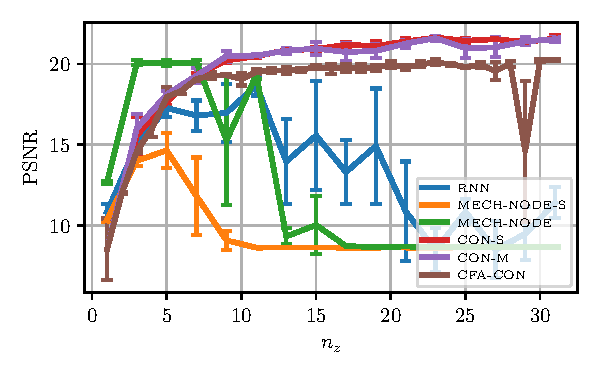
\includegraphics[width=0.49\textwidth, trim={5, 5, 5, 5}]{con/figures/results/latent_dynamics/pcc_ns-2/sweep_psnr_rec_dynamic_vs_n_z.pdf}}
    \subfigure[PSNR vs. model parameters]{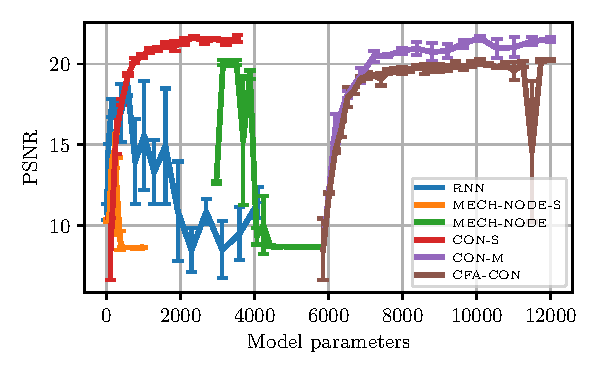
\includegraphics[width=0.49\textwidth, trim={5, 5, 5, 5}]{con/figures/results/latent_dynamics/pcc_ns-2/sweep_psnr_rec_dynamic_vs_num_trainable_params.pdf}}
    \\
    \subfigure[SSIM vs. latent dimension $n_z$]{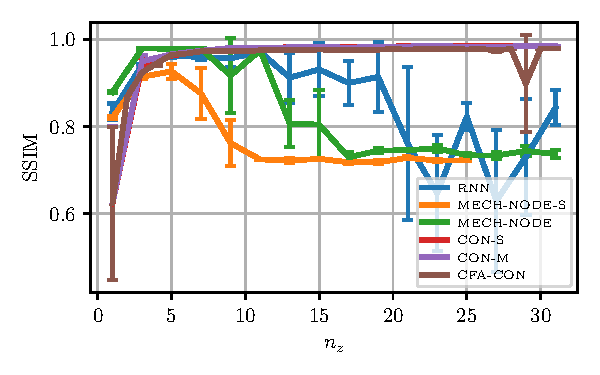
\includegraphics[width=0.49\textwidth, trim={5, 5, 5, 5}]{con/figures/results/latent_dynamics/pcc_ns-2/sweep_ssim_rec_dynamic_vs_n_z.pdf}}
    \subfigure[SSIM vs. model parameters]{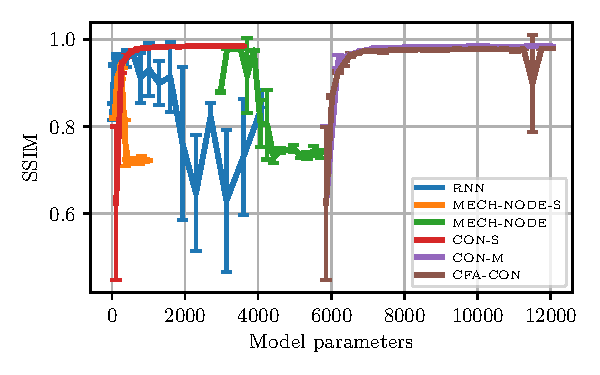
\includegraphics[width=0.49\textwidth, trim={5, 5, 5, 5}]{con/figures/results/latent_dynamics/pcc_ns-2/sweep_ssim_rec_dynamic_vs_num_trainable_params.pdf}}
    \caption{Evaluation of prediction performance of the various models vs. the dimension of their latent representation $n_z$ and the number of trainable parameters of the dynamics model, respectively. We optimize the hyperparameters for the case of $n_z=8$, and execute the tuning separately for each model and dataset.}
    \label{fig:apx-con:latent_dynamics_sweep_pcc_ns-2}
\end{figure}

\begin{figure}
    \centering
    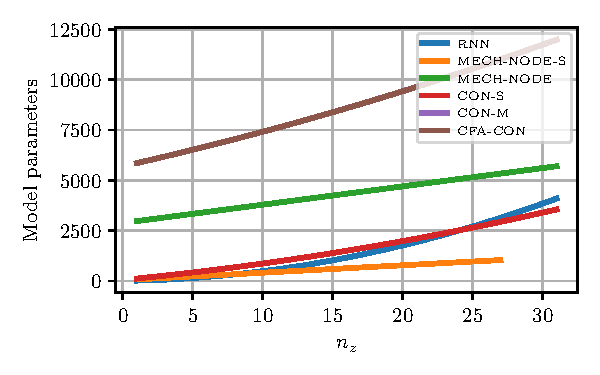
\includegraphics[width=0.6\columnwidth]{con/figures/results/latent_dynamics/pcc_ns-2/sweep_num_trainable_params_vs_n_z.pdf}
    \caption{Plot of number of trainable parameters vs. the latent dimension $n_z$ of various models trained on the \emph{PCC-NS-2} dataset. As we have configured them, \emph{CON-M} and \emph{CFA-CON} always have the same number of parameters (i.e., overlaying lines).}
    \label{fig:apx-con:num_trainable_params_vs_n_z}
\end{figure}

\begin{figure}[hb]
    \centering
    \subfigure{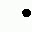
\includegraphics[width=0.160\columnwidth]{con/figures/results/latent_dynamics/s-p+f/sequence_of_stills/rollout_6_target_0.00.png}}
    \subfigure{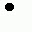
\includegraphics[width=0.160\columnwidth]{con/figures/results/latent_dynamics/s-p+f/sequence_of_stills/rollout_6_target_0.55.png}}
    \subfigure{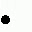
\includegraphics[width=0.160\columnwidth]{con/figures/results/latent_dynamics/s-p+f/sequence_of_stills/rollout_6_target_1.10.png}}
    \subfigure{
\includegraphics[width=0.160\columnwidth]{con/figures/results/latent_dynamics/s-p+f/sequence_of_stills/rollout_6_target_1.65.png}}
    \subfigure{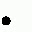
\includegraphics[width=0.160\columnwidth]{con/figures/results/latent_dynamics/s-p+f/sequence_of_stills/rollout_6_target_2.20.png}}
    \subfigure{
\includegraphics[width=0.160\columnwidth]{con/figures/results/latent_dynamics/s-p+f/sequence_of_stills/rollout_6_target_2.75.png}}
    \\
    \setcounter{subfigure}{0}
    \subfigure[t=\SI{0.0}{s}]{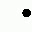
\includegraphics[width=0.160\columnwidth]{con/figures/results/latent_dynamics/s-p+f/sequence_of_stills/rollout_6_pred_0.00.png}}
    \subfigure[t=\SI{0.55}{s}]{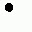
\includegraphics[width=0.160\columnwidth]{con/figures/results/latent_dynamics/s-p+f/sequence_of_stills/rollout_6_pred_0.55.png}}
    \subfigure[t=\SI{1.10}{s}]{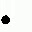
\includegraphics[width=0.160\columnwidth]{con/figures/results/latent_dynamics/s-p+f/sequence_of_stills/rollout_6_pred_1.10.png}}
    \subfigure[t=\SI{1.65}{s}]{
\includegraphics[width=0.160\columnwidth]{con/figures/results/latent_dynamics/s-p+f/sequence_of_stills/rollout_6_pred_1.65.png}}
    \subfigure[t=\SI{2.20}{s}]{
\includegraphics[width=0.160\columnwidth]{con/figures/results/latent_dynamics/s-p+f/sequence_of_stills/rollout_6_pred_2.20.png}}
    \subfigure[t=\SI{2.75}{s}]{
\includegraphics[width=0.160\columnwidth]{con/figures/results/latent_dynamics/s-p+f/sequence_of_stills/rollout_6_pred_2.75.png}}
    \caption{Prediction sequence of a \gls{CON} model with latent dimension $n_z=4$ trained on the single pendulum with friction (\emph{S-P+F}) dataset~\cite{botev2021priors}. 
    \textbf{Top row:} Ground-truth evolution of the system. \textbf{Bottom row:} Predictions of the \emph{CON} model. \newline
    The prediction model is given three images centered around $t=0$ for encoding the initial latent $z(0)$ and estimation of the initial latent velocity $\dot{z}(0)$. Subsequently, we roll out the autonomous network dynamics (i.e., unforced) and compare the decoded predictions with the ground-truth evolution of the system.  
    }\label{fig:apx-con:latent_dynamics:sequence_of_stills:s-p+f:rollout6}
\end{figure}

\begin{figure}[hb]
    \centering
    \subfigure{
\includegraphics[width=0.160\columnwidth]{con/figures/results/latent_dynamics/cs/sequence_of_stills/rollout_19_target_0.00.png}}
    \subfigure{
\includegraphics[width=0.160\columnwidth]{con/figures/results/latent_dynamics/cs/sequence_of_stills/rollout_19_target_0.04.png}}
    \subfigure{
\includegraphics[width=0.160\columnwidth]{con/figures/results/latent_dynamics/cs/sequence_of_stills/rollout_19_target_0.08.png}}
    \subfigure{
\includegraphics[width=0.160\columnwidth]{con/figures/results/latent_dynamics/cs/sequence_of_stills/rollout_19_target_0.12.png}}
    \subfigure{
\includegraphics[width=0.160\columnwidth]{con/figures/results/latent_dynamics/cs/sequence_of_stills/rollout_19_target_0.16.png}}
    \subfigure{
\includegraphics[width=0.160\columnwidth]{con/figures/results/latent_dynamics/cs/sequence_of_stills/rollout_19_target_0.20.png}}
    \\
    \setcounter{subfigure}{0}
    \subfigure[t=\SI{0.00}{s}]{
\includegraphics[width=0.160\columnwidth]{con/figures/results/latent_dynamics/cs/sequence_of_stills/rollout_19_pred_0.00.png}}
    \subfigure[t=\SI{0.04}{s}]{
\includegraphics[width=0.160\columnwidth]{con/figures/results/latent_dynamics/cs/sequence_of_stills/rollout_19_pred_0.04.png}}
    \subfigure[t=\SI{0.08}{s}]{
\includegraphics[width=0.160\columnwidth]{con/figures/results/latent_dynamics/cs/sequence_of_stills/rollout_19_pred_0.08.png}}
    \subfigure[t=\SI{0.12}{s}]{
\includegraphics[width=0.160\columnwidth]{con/figures/results/latent_dynamics/cs/sequence_of_stills/rollout_19_pred_0.12.png}}
    \subfigure[t=\SI{0.16}{s}]{
\includegraphics[width=0.160\columnwidth]{con/figures/results/latent_dynamics/cs/sequence_of_stills/rollout_19_pred_0.16.png}}
    \subfigure[t=\SI{0.20}{s}]{
\includegraphics[width=0.160\columnwidth]{con/figures/results/latent_dynamics/cs/sequence_of_stills/rollout_19_pred_0.20.png}}
    \caption{Prediction sequence of a forced \gls{CON} model with latent dimension $n_z=12$ trained on the soft robotic \emph{CS} dataset containing trajectories of a simulated constant strain robot with one segment. 
    \textbf{Top row:} Ground-truth evolution of the system. \textbf{Bottom row:} Predictions of the \emph{CON-M} model. \newline
    The prediction model is given three images centered around $t=0$ for encoding the initial latent $z(0)$ and estimation of the initial latent velocity $\dot{z}(0)$. Subsequently, we roll out the autonomous network dynamics (i.e., unforced) and compare the decoded predictions with the ground-truth evolution of the system.  
    }\label{fig:apx-con:latent_dynamics:sequence_of_stills:cs:rollout19}
\end{figure}


\begin{figure}[hb]
    \centering
    % image size: 575x575px
    \subfigure{
\includegraphics[width=0.192\columnwidth]{con/figures/results/latent_dynamics/pcc_ns-2/sequence_of_stills/rollout2-0001_gt.png}}
    \subfigure{
\includegraphics[width=0.192\columnwidth]{con/figures/results/latent_dynamics/pcc_ns-2/sequence_of_stills/rollout2-0002_gt.png}}
    \subfigure{
\includegraphics[width=0.192\columnwidth]{con/figures/results/latent_dynamics/pcc_ns-2/sequence_of_stills/rollout2-0003_gt.png}}
    \subfigure{
\includegraphics[width=0.192\columnwidth]{con/figures/results/latent_dynamics/pcc_ns-2/sequence_of_stills/rollout2-0004_gt.png}}
    \subfigure{
\includegraphics[width=0.192\columnwidth]{con/figures/results/latent_dynamics/pcc_ns-2/sequence_of_stills/rollout2-0005_gt.png}}
    \\
    \setcounter{subfigure}{0}
    \subfigure[t=\SI{0.0}{s}]{
\includegraphics[width=0.192\columnwidth]{con/figures/results/latent_dynamics/pcc_ns-2/sequence_of_stills/rollout2-0001_pred.png}}
    \subfigure[t=\SI{0.3}{s}]{
\includegraphics[width=0.192\columnwidth]{con/figures/results/latent_dynamics/pcc_ns-2/sequence_of_stills/rollout2-0002_pred.png}}
    \subfigure[t=\SI{0.6}{s}]{
\includegraphics[width=0.192\columnwidth]{con/figures/results/latent_dynamics/pcc_ns-2/sequence_of_stills/rollout2-0003_pred.png}}
    \subfigure[t=\SI{0.9}{s}]{
\includegraphics[width=0.192\columnwidth]{con/figures/results/latent_dynamics/pcc_ns-2/sequence_of_stills/rollout2-0004_pred.png}}
    \subfigure[t=\SI{1.2}{s}]{
\includegraphics[width=0.192\columnwidth]{con/figures/results/latent_dynamics/pcc_ns-2/sequence_of_stills/rollout2-0005_pred.png}}
    \caption{Prediction sequence of an unforced \gls{CON} model with latent dimension $n_z=8$ trained on the \emph{PCC-NS-2} dataset. 
    \textbf{Top row:} Ground-truth evolution of the system. \textbf{Bottom row:} Predictions of the \emph{CON-M} model. \newline
    The prediction model is given three images centered around $t=0$ for encoding the initial latent $z(0)$ and estimation of the initial latent velocity $\dot{z}(0)$. Subsequently, we roll out the autonomous network dynamics (i.e., unforced) and compare the decoded predictions with the ground-truth evolution of the system.  
    }\label{fig:apx-con:latent_dynamics:sequence_of_stills:pcc_ns-2:rollout2}
\end{figure}

\begin{figure}[hb]
    \centering
    % image size: 575x575px
    \subfigure{
\includegraphics[width=0.192\columnwidth]{con/figures/results/latent_dynamics/pcc_ns-2/sequence_of_stills/rollout1-0001_gt.png}}
    \subfigure{
\includegraphics[width=0.192\columnwidth]{con/figures/results/latent_dynamics/pcc_ns-2/sequence_of_stills/rollout1-0002_gt.png}}
    \subfigure{
\includegraphics[width=0.192\columnwidth]{con/figures/results/latent_dynamics/pcc_ns-2/sequence_of_stills/rollout1-0003_gt.png}}
    \subfigure{
\includegraphics[width=0.192\columnwidth]{con/figures/results/latent_dynamics/pcc_ns-2/sequence_of_stills/rollout1-0004_gt.png}}
    \subfigure{
\includegraphics[width=0.192\columnwidth]{con/figures/results/latent_dynamics/pcc_ns-2/sequence_of_stills/rollout1-0005_gt.png}}
    \\
    \setcounter{subfigure}{0}
    \subfigure[t=\SI{0.0}{s}]{
\includegraphics[width=0.192\columnwidth]{con/figures/results/latent_dynamics/pcc_ns-2/sequence_of_stills/rollout1-0001_pred.png}}
    \subfigure[t=\SI{0.3}{s}]{
\includegraphics[width=0.192\columnwidth]{con/figures/results/latent_dynamics/pcc_ns-2/sequence_of_stills/rollout1-0002_pred.png}}
    \subfigure[t=\SI{0.6}{s}]{
\includegraphics[width=0.192\columnwidth]{con/figures/results/latent_dynamics/pcc_ns-2/sequence_of_stills/rollout1-0003_pred.png}}
    \subfigure[t=\SI{0.9}{s}]{
\includegraphics[width=0.192\columnwidth]{con/figures/results/latent_dynamics/pcc_ns-2/sequence_of_stills/rollout1-0004_pred.png}}
    \subfigure[t=\SI{1.2}{s}]{
\includegraphics[width=0.192\columnwidth]{con/figures/results/latent_dynamics/pcc_ns-2/sequence_of_stills/rollout1-0005_pred.png}}
    \caption{Prediction sequence of a forced \gls{CON} model with latent dimension $n_z=8$ trained on the \emph{PCC-NS-2} dataset. 
    \textbf{Top row:} Ground-truth evolution of the system. \textbf{Bottom row:} Predictions of the \emph{CON-M} model. \newline
    The prediction model is given three images centered around $t=0$ for encoding the initial latent $z(0)$ and estimation of the initial latent velocity $\dot{z}(0)$. Subsequently, we provide the same constant input $u$ to both the simulator and the network dynamics (i.e., unforced) and compare the decoded predictions with the ground-truth evolution of the system.  
    }\label{fig:apx-con:latent_dynamics:sequence_of_stills:pcc_ns-2:rollout1}
\end{figure}